\subsection{Superthreshold Operation}

When we continue to increase the gate voltage, we attract more and more free electrons to the surface of the channel. Once they become the majority carriers in the channel, the channel becomes n-type and is said to be inverted. We operate in the superthreshold regime now. In the superthreshold regime, the electrical field becomes so strong that it is the main cause for the current flow and makes the previously calculated diffusion current negligible. Remember that the drift current caused by an electrical field is determined by the following equation:

\begin{equation}
    I = q n \mu \epsilon W t\label{eq:electrical_field}
\end{equation}

where $q$ is the electron charge, $n$ the carrier concentration, $\mu$ the mobility of electrons, $\epsilon$ the electrical field and $W$ and $t$ the width and the depth of the channel respectively. In the previous section, we have seen that the charge $Q_i$ that accumulates in the inversion region of our channel is dependent on the channel's MOS structure.

\begin{equation}
    Q_i = C_{ox} (V_g - V_T)
\end{equation}

We can express our charge concentration $qn$ in terms of $Q_i$.

\begin{equation}
    qn = \frac{Q_i}{t}
\end{equation}

Note that $Q_i$ is the inversion charge per unit area. For simplicity we assume that our electrical field is constant. We can therefore simply express $\epsilon$ by the voltage difference across the channel.

\begin{equation}
    \epsilon = \frac{V_d - V_s}{L}
\end{equation}

where L is the length of the channel. Substituting these relationships into our equation for the drift current \eqref{eq:electrical_field} yields our current equation in superthreshold.

\begin{equation}
    I = C_{ox} (V_g - V_T) \mu \frac{V_d - V_s}{L} W = \beta (V_g - V_T) (V_d - V_s) 
\end{equation}

where $\beta = \mu C_{ox} \frac{W}{L}$. Assuming that $\beta$ and $V_{ds}$ are constant, we can see that there is a linear relationship between the current $I_{ds}$ and the gate voltage $V_{gs}$. This relationship is also demonstrated in figure \ref{fig:super_small_vds}.\\

\begin{figure}
    \centering
    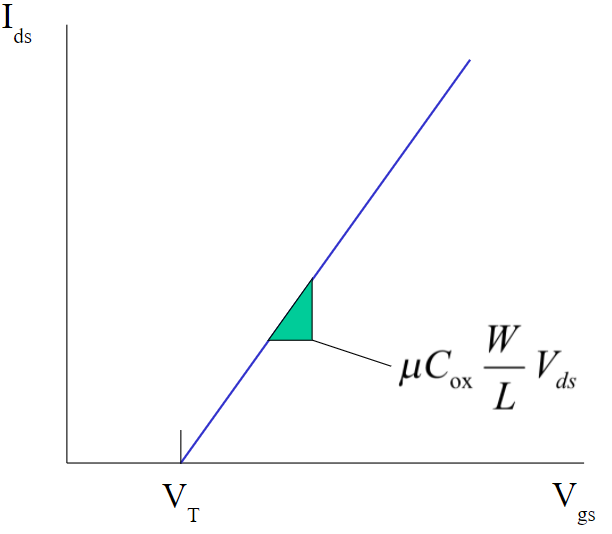
\includegraphics[width=.5\linewidth]{Figures/superthreshold_small_vds.PNG}
    \caption{Relationship between the gate voltage $V_{gs}$ and the current $I_{ds}$ for small values of $V_{ds}$.}
    \label{fig:super_small_vds}
\end{figure}

\textbf{Effective Threshold Voltage}\\

In order to switch between the sub- and the superthreshold regime, we have to increase our gate voltage until it crosses a specific voltage value, the threshold voltage $V_T$. So far, we have assumed that $V_T$ is a fixed value, however in reality this is not the case. When we increase the source voltage, hence decreasing the voltage difference $V_{ds}$, our current decreases as a consequence of the increased energy barrier between the source and the channel. How much do we have to change our gate voltage to retrieve our original current? An increase of $V_s$ can be counter balanced by an increase of $\phi_s$. For $\Delta V_s = \Delta \phi_s$, our energy barrier, and hence the generated current, remains the same. Remember that $\frac{\Delta \phi_s}{\Delta V_G} = \kappa$, so we have to increase our gate voltage by a factor of $\frac{1}{\kappa}$ more than the source voltage. But what does this have to do with the threshold voltage? At the threshold point, electrons become the majority carriers in the channel. These mobile electrons are mainly attracted from the source. For increasing $V_s$, we therefore have to increase our gate voltage by the factor of $\frac{1}{\kappa}$ more in order to attract enough free carriers to invert our channel. The actual, \textbf{effective}, threshold voltage is hence dependent on the source voltage.

\begin{equation}
    V_T = V_{T0} + \frac{V_s}{\kappa}\label{eq:effective_threshold}
\end{equation}

Let's have a look at our channel again. We have previously assumed that the inversion charge $Q_i$ is constant along the channel. In reality, it decreases from its highest concentration at the source end to its lowest concentration at the drain end. The charge is dependent on the threshold voltage at the channel ends and consequently on the source and drain voltages as given by \eqref{eq:effective_threshold}. For the charge at the source and the drain end we get:

\begin{equation}
    Q_s = C_{ox} (V_g - V_T) = C_{ox} (V_g - V_{T0} - \frac{V_s}{\kappa})
\end{equation}

\begin{equation}
    Q_d = C_{ox} (V_g - V_T) = C_{ox} (V_g - V_{T0} - \frac{V_d}{\kappa})
\end{equation}

So for a constant gate voltage, the charge decreases for an increasing $V_s$ and $V_d$. As $V_d > V_s$, the charge concentration at the drain end is indeed lower just as expected. If we continue to increase $V_d$, the charge at the drain end of the channel $Q_d$ will decrease until it eventually becomes zero. The channel is said to be "pinched off". Figure \ref{fig:channel_shape_vds} demonstrates how the channel shape changes for different values of $V_{ds}$. The so-called pinchoff point is the point in the channel where the inversion charge appears first. The electrons are moved from the drain end into the drain region by the electrical field between the drain and the channel. The drain voltage, however, does not influence the current, i.e. the electron movement from the source along the channel, anymore and $I_{ds}$ remains constant for increasing values of $V_{ds}$. Similar to the subthreshold regime, we now say that the current is saturated and that we operate in the saturation region. This happens once the voltage difference $V_{ds}$ corresponds to the overdrive voltage $V_{ov}$, so when the charge difference equals the charge concentration at the source. For simplicity, we assume a fixed threshold value again and get the following saturation voltage:

\begin{equation}
    V_{ds,sat} = V_{gs} - V_T = V_{ov}
\end{equation}

By replacing $V_{ds}$ with $V_{ds,sat}$, we can define the saturated current $I_{ds,sat}$ .

\begin{equation}
    \frac{1}{2} \beta (V_{gs} - V_T)^2 = \frac{1}{2} \beta V_{ov} ^2
\end{equation}

\begin{figure}
    \centering
    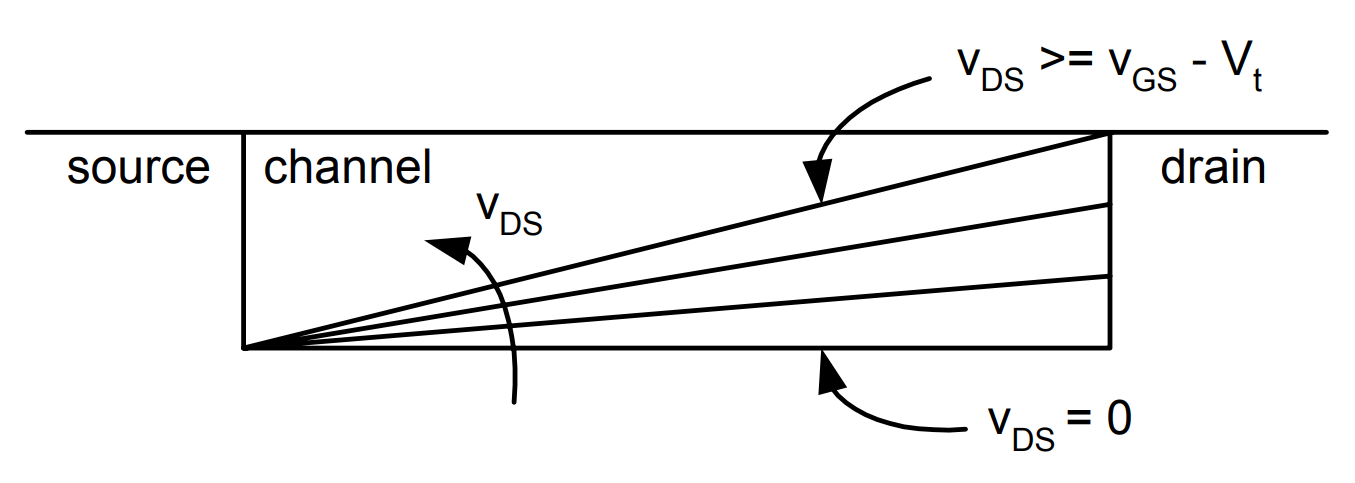
\includegraphics[width=.8\linewidth]{Figures/channel_shape_vds.PNG}
    \caption{Different channel shapes for different values of $V_{ds}$ [Taken from \url{http://in.ncu.edu.tw/ncume_ee/harvard-es154/lect_12_MOSFETs.pdf}].}
    \label{fig:channel_shape_vds}
\end{figure}

The additional factor $\frac{1}{2}$ can be explained by a more detailed derivation of the drain current $I_{ds}$ which does not assume a constant electrical field along the channel. Please refer to \cite{liu2002analog} if you want to find out more. Figure \ref{fig:superthreshold_ohmic_saturation} visualizes the relationship between $V_{ds}$ and $I_{ds}$ for different gate voltage $V_{gs}$.\\

\begin{figure}
    \centering
    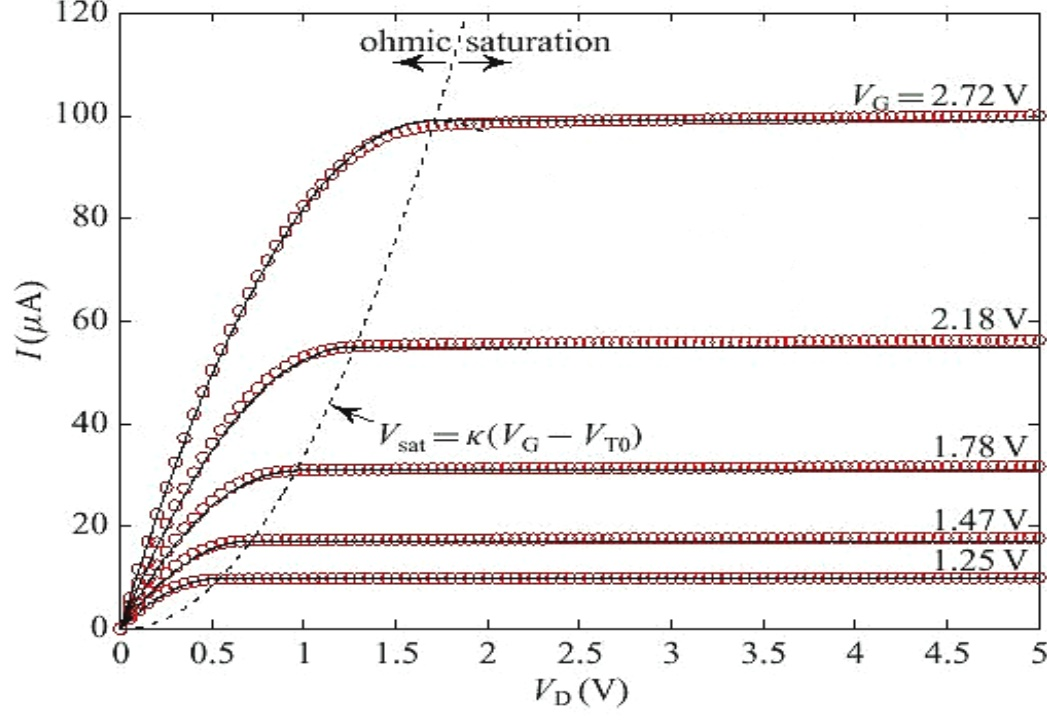
\includegraphics[width=.8\linewidth]{Figures/superthreshold_ohmic_saturation.jpg}
    \caption{Relationship between $V_{ds}$ and $I_{ds}$ for different gate voltage $V_{gs}$.}
    \label{fig:superthreshold_ohmic_saturation}
\end{figure}

\textbf{Special current $I_s$}\\

Finally, let's define a specific current you should know about: the special current $I_s$. It defines the border between weak and strong inversion and is particularly useful during designing. It approximately corresponds to the current at the overdrive voltage $V_{ov} = U_T$.

\begin{equation}
    I_s = 2 \mu C_{ox} \frac{W}{L} U_T^2 = 2 \beta U_T^2
\end{equation}\\

Let's sum up the equations we derived for an nFET transistor in superthreshold regime.\\

\textbf{Superthreshold nFET $I_{ds}$ current}
\begin{itemize}
    \item Triode/ Linear/ Ohmic Region
    \begin{equation}
        I_{ds} = \beta (V_{gs} - V_T) V_{ds} = \beta V_{ov} V_{ds}
    \end{equation}
    \item Saturation Region
    \begin{equation}
        I_{ds} = \frac{1}{2} \beta (V_{gs} - V_T)^2 = \frac{1}{2} \beta V_{ov}^2
    \end{equation}
\end{itemize}